\section{Materials and Methods}
\label{sec:methods}

This section defines the graph-classification task, the Matrix-Residual architecture family, the benchmark protocol, the synthetic structural stress test, and the mechanism metrics. The guiding principle is to isolate residual topology while holding the remaining learning pipeline fixed.

\subsection{Problem definition and notation}

Let \(\mathcal{G}=(\mathcal{V},\mathcal{E})\) be a graph with node feature matrix \(\mathbf{X}\in\mathbb{R}^{n\times d_{\mathrm{in}}}\) and adjacency structure \(\mathbf{A}\). For a dataset \(\mathcal{D}=\{(\mathcal{G}_i,y_i)\}_{i=1}^{N}\), the objective is to learn \(f_{\theta}:\mathcal{G}\rightarrow \hat{y}\), where \(\hat{y}\) is the predicted graph label.

The compared model families share the same graph-classification wrapper:
\begin{itemize}
    \item \textbf{Plain}: stacked message passing without explicit residual reuse.
    \item \textbf{VerticalRes}: same-branch residual reuse from the previous layer.
    \item \textbf{HorizontalRes}: cross-branch exchange between adjacent branches at the same depth.
    \item \textbf{MatrixRes}: local two-dimensional reuse over vertical, horizontal, and diagonal neighbors.
    \item \textbf{MatrixResGated}: matrix reuse with gated or sparse residual filtering.
\end{itemize}

\subsection{Shared graph-classification pipeline}

Let \(B\) be the number of branches and \(L\) be the number of message-passing layers. The hidden state at branch \(b\) and layer \(\ell\) is written as \(\mathbf{H}^{(\ell)}_{b}\), where \(b\in\{1,\ldots,B\}\). A branch-local propagation step is
\begin{equation}
\mathbf{Z}^{(\ell)}_{b} = \phi^{(\ell)}_{b}\left(\mathbf{H}^{(\ell-1)}_{b}, \mathbf{A}\right),
\end{equation}
where \(\phi\) is instantiated as one of four standard operators: GCNConv \cite{kipf2017gcn}, GATConv \cite{velivckovic2017graph}, SAGEConv \cite{hamilton2017inductive}, or GINConv \cite{xu2019gin}. The residual-enhanced update is
\begin{equation}
\mathbf{H}^{(\ell)}_{b} =
\mathbf{Z}^{(\ell)}_{b} +
\sum_{(b',\ell')\in\mathcal{N}(b,\ell)}
\mathcal{R}_{(b',\ell')\rightarrow(b,\ell)}
\left(\mathbf{H}^{(\ell')}_{b'}\right).
\end{equation}
The only term that changes across architectures is the residual neighborhood \(\mathcal{N}(b,\ell)\) and the residual transform \(\mathcal{R}\).

After the final message-passing layer, each branch is pooled to a graph-level vector by global mean pooling and the branch vectors are combined before classification. We intentionally avoid architecture-specific pooling heads such as differentiable pooling or self-attention pooling \cite{ying2018hierarchical,lee2019self}, because the purpose is to isolate residual topology rather than to compare readout mechanisms. The classifier is trained with cross-entropy loss. Figure~\ref{fig:architecture} summarizes the shared pipeline and the residual routes compared in the study.

\begin{figure}[!htbp]
\centering
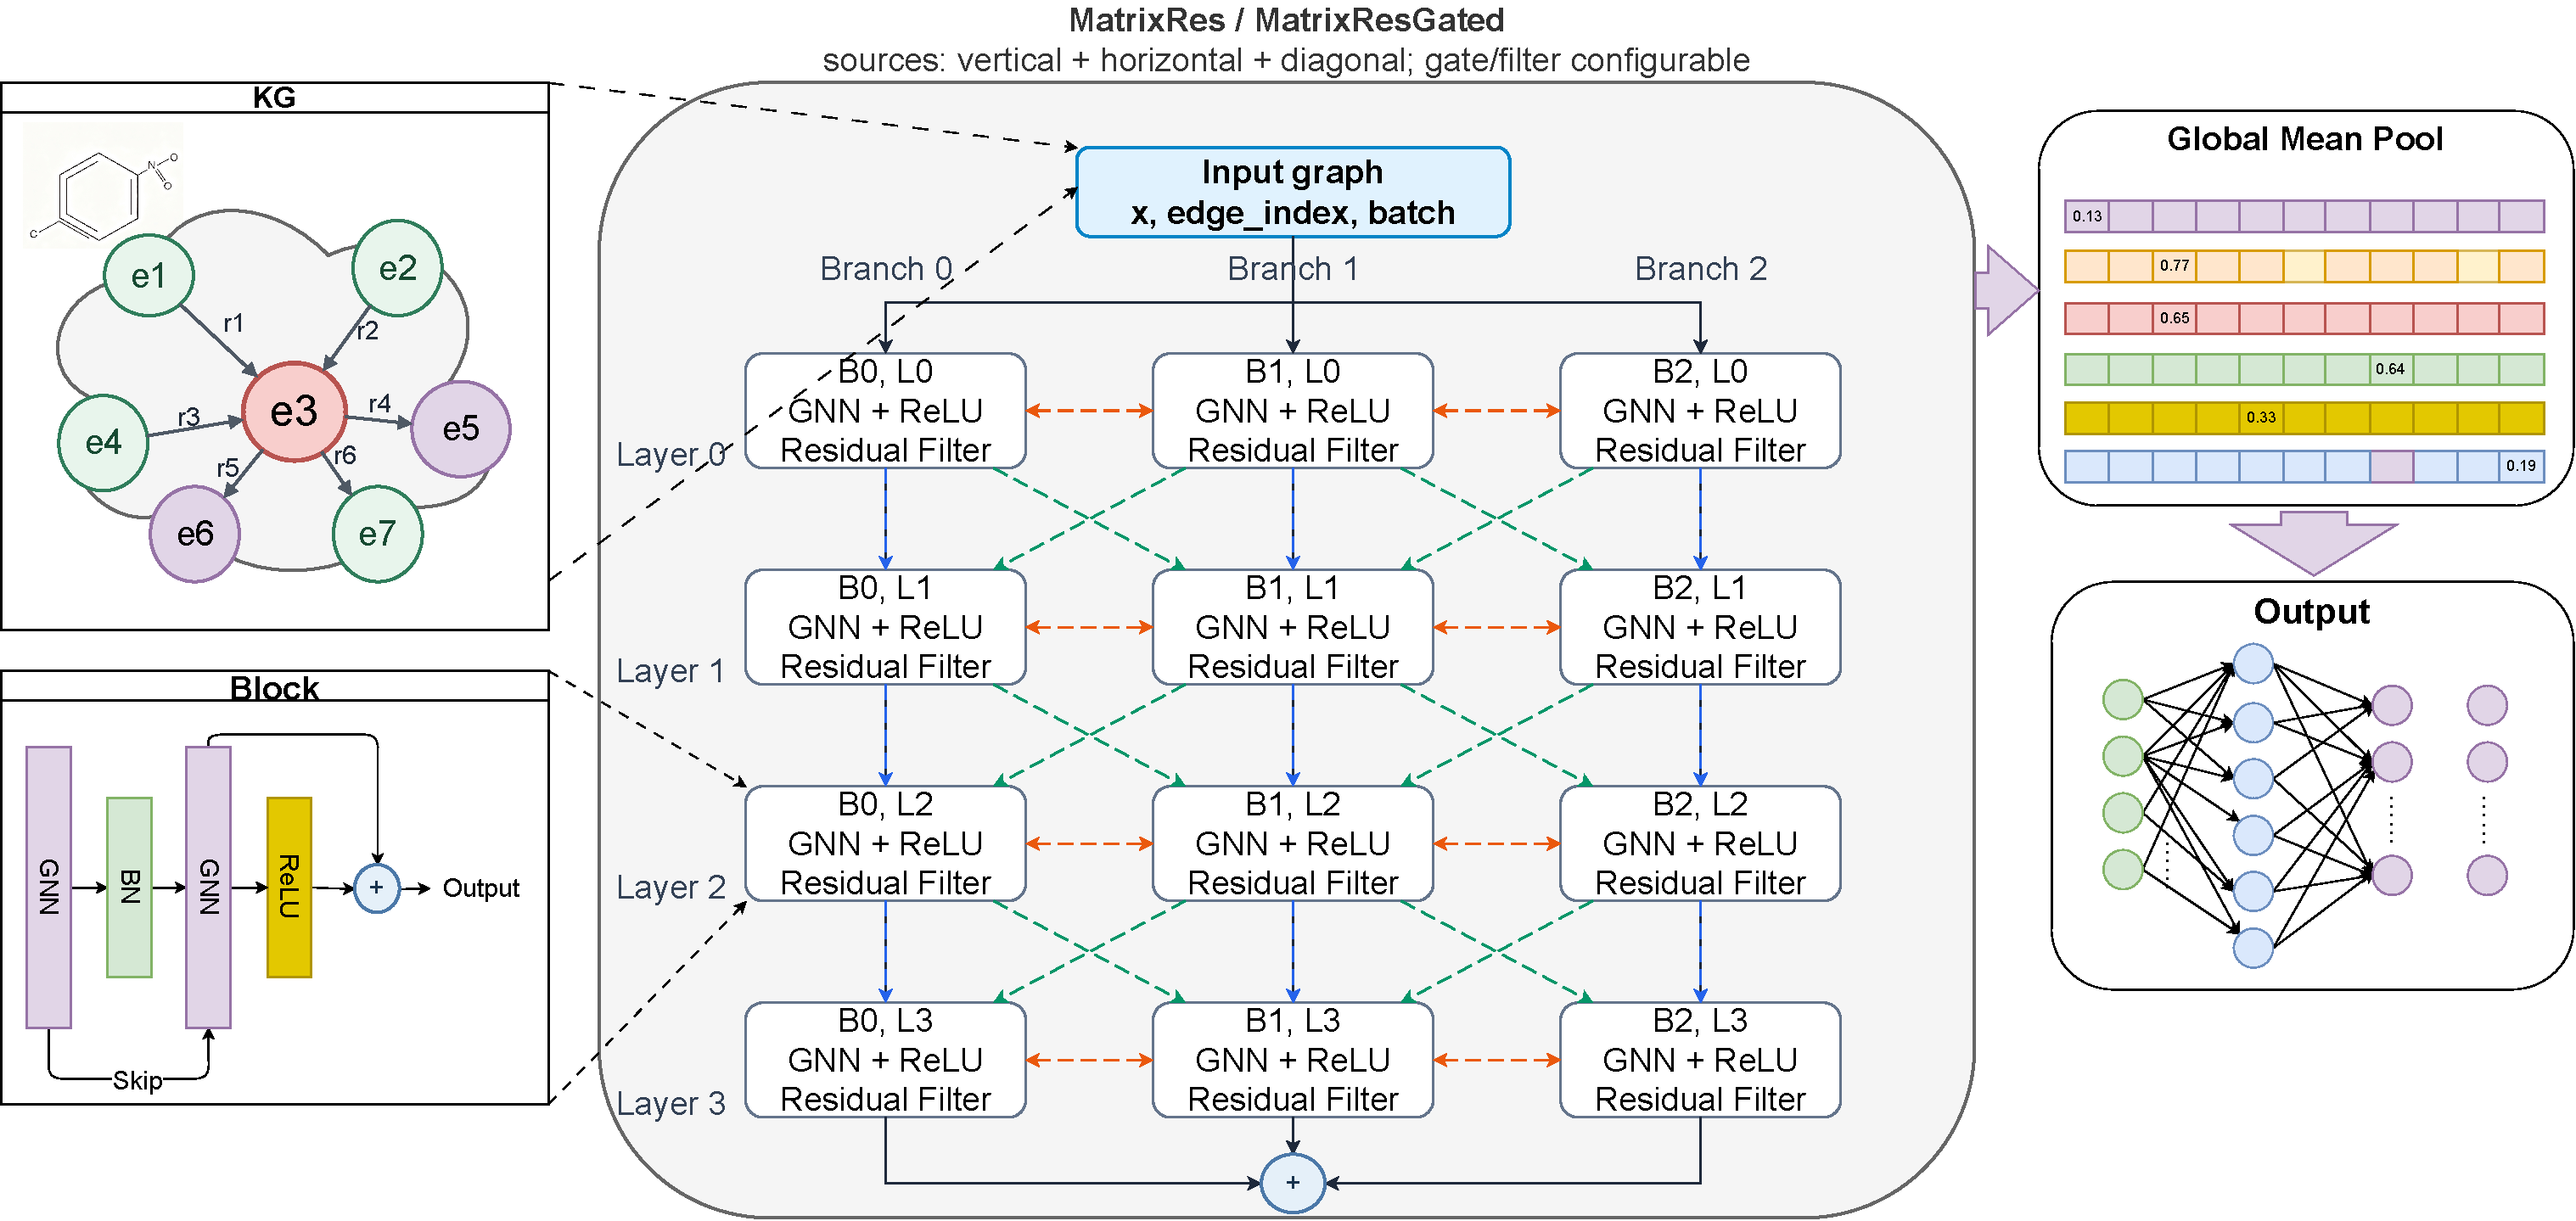
\includegraphics[width=0.95\linewidth]{figures/cr_gnn_graph_architecture.pdf}
\caption{Architecture overview of the compared residual neighborhoods on the branch-by-layer grid. The same message-passing backbone and graph-level readout are kept fixed while the residual routes are changed.}
\label{fig:architecture}
\end{figure}

\subsection{Residual neighborhoods}
\label{sec:model}

\textbf{Plain.} The plain baseline has no residual neighborhood:
\begin{equation}
\mathcal{N}(b,\ell)=\emptyset.
\end{equation}

\textbf{VerticalRes.} Vertical residual reuse injects the previous layer on the same branch:
\begin{equation}
\mathcal{N}(b,\ell)=\{(b,\ell-1)\}.
\end{equation}

\textbf{HorizontalRes.} Horizontal residual reuse exchanges information across adjacent branches at the same depth:
\begin{equation}
\mathcal{N}(b,\ell)=\{(b-1,\ell),(b+1,\ell)\},
\end{equation}
with boundary branches using only valid neighbors. When \(B=1\), this horizontal neighborhood is empty.

\textbf{MatrixRes.} Matrix residual reuse combines vertical, horizontal, and diagonal neighborhoods:
\begin{equation}
\mathcal{N}(b,\ell)=
\{(b,\ell-1),(b-1,\ell),(b+1,\ell),(b-1,\ell-1),(b+1,\ell-1)\}.
\end{equation}
This local stencil is intentionally not dense all-to-all mixing. It preserves an interpretable residual structure over the branch-by-layer grid. Invalid boundary neighbors are removed; therefore, when \(B=1\), MatrixRes keeps the same-branch vertical residual path after the first layer but has no branch-neighbor routes.

\textbf{MatrixResGated.} MatrixResGated uses the same neighborhood as MatrixRes, but the residual transform controls the injected signal:
\begin{equation}
\mathcal{R}(\mathbf{U}) =
\begin{cases}
\alpha \mathbf{U}, & \text{identity residual filtering with a gate},\\
\alpha\,\mathrm{softshrink}_{\lambda}(\mathbf{U}), & \text{sparse residual filtering with a gate}.
\end{cases}
\end{equation}
In the main benchmark, Plain, VerticalRes, HorizontalRes, and MatrixRes use identity residual filtering. MatrixResGated uses sparse residual filtering with \(\lambda=0.05\) and a learnable scalar gate initialized at 0.8. When \(B=1\), MatrixResGated still applies gated sparse filtering to the remaining matrix-residual paths. The implementation also supports top-\(k\) residual filtering and fixed gates, but these are not the default settings used for the main reported results.

\subsection{Datasets and sources}
\label{sec:datasets}

The main benchmark uses six third-party datasets from TUDataset \cite{morris2020tudataset}: PROTEINS, DD, ENZYMES, MUTAG, AIDS, and Mutagenicity. The TUDataset collection is available at \url{https://chrsmrrs.github.io/datasets/} and is accessed through PyTorch Geometric \cite{fey2019fast}. PROTEINS and DD are binary protein-structure graph classification benchmarks, ENZYMES is a six-class enzyme classification benchmark, and MUTAG, AIDS, and Mutagenicity provide supplementary molecular-graph robustness checks. All experiments use the raw benchmark features and graph structures without task-specific feature engineering, graph augmentation, or edge redesign.

\subsection{Data preprocessing}

The preprocessing pipeline is intentionally minimal to keep the comparison focused on residual topology. TUDataset graphs are loaded with their provided node features and graph labels. The code does not add handcrafted chemical or biological descriptors, does not perform graph augmentation, and does not rewire edges. Synthetic graphs are generated from controlled structural parameters, assigned generic eight-dimensional node features derived from normalized degree and random feature channels, and then passed to the same graph-classification pipeline. For every dataset, graph-level folds are fixed by the experiment scripts so that all compared residual topologies use matched train, validation, and test splits.

\subsection{Technique selection}

The implemented techniques were selected to isolate one architectural factor: residual information flow in a multi-branch GNN. GCNConv, GATConv, SAGEConv, and GINConv were chosen because they are canonical message-passing operators representing spectral-style convolution, attention-based aggregation, neighborhood sampling/aggregation, and injective multiset aggregation. Plain, VerticalRes, HorizontalRes, MatrixRes, and MatrixResGated were then compared under the same operators, pooling, classifier, and fold protocol. This selection makes the residual-topology question testable without mixing it with unrelated changes in readout design, feature engineering, or task-specific model tuning.

\subsection{Evaluation protocol and metrics}

All main results use graph-level five-fold evaluation. For fold \(k\), the test accuracy is
\begin{equation}
\mathrm{Acc}_{k}=
\frac{1}{|\mathcal{T}_{k}|}
\sum_{(\mathcal{G}_{i},y_{i})\in\mathcal{T}_{k}}
\mathbf{1}[\hat{y}_{i}=y_{i}].
\end{equation}
Across folds, we report
\begin{equation}
\overline{\mathrm{Acc}}=\frac{1}{5}\sum_{k=1}^{5}\mathrm{Acc}_{k},
\end{equation}
and the fold-level standard deviation.

Accuracy is the primary metric because every benchmark is a graph-level classification task with discrete labels and because it is the standard summary reported for the selected TUDataset tasks. The fold-level standard deviation is reported to expose variability across train/test splits. For the synthetic multi-class benchmark, macro-F1 is added because it gives equal weight to each class, and chance-normalized accuracy is added because raw accuracy is not directly comparable when the number of classes changes from two to eight. Mechanism metrics such as branch diversity, cosine similarity, CKA, residual activity, and gradient norm are used as diagnostic measurements rather than as optimization targets.

\subsection{Synthetic multi-class structural benchmark}
\label{sec:synthetic}

To test residual topology under controlled structural class granularity, we add a synthetic benchmark based on five graph families: Bernoulli random graphs recorded as ER, Barabási--Albert (BA) graphs, stochastic block models (SBM), Watts--Strogatz (WS) graphs, and a regular-degree control. For each family, we generate seven multi-class datasets with class counts \(C\in\{2,3,4,5,6,7,8\}\). Each class contains 200 graphs, so each dataset contains \(200C\) graphs. Graph sizes are sampled between 30 and 80 nodes, and every node receives an eight-dimensional feature vector derived from normalized degree and random feature channels. The features are intentionally generic and do not encode the class label directly.

The synthetic labels are controlled by family-specific structural parameters. The ER identifier in our experiment records corresponds strictly to Gilbert's \(G(n,p)\) model: each node pair is connected independently with Bernoulli probability \(p\), producing sparse random structures at different densities \cite{gilbert1959random}. BA classes differ by the preferential-attachment count and provide long-tailed degree structures \cite{barabasi1999emergence}. SBM classes vary the within-block and between-block probabilities to control community separation \cite{holland1983stochastic}. WS classes differ by rewiring probability and provide small-world structures with local clustering and short paths \cite{watts1998collective}. The regular-degree control uses randomly relabeled regular ring lattices with different fixed degrees. It provides degree-uniform structures but is not sampled from the uniform random-regular distribution, for which \cite{wormald1999models} provides background. These families are used as stress tests rather than as replacements for real graph-classification benchmarks.

The synthetic benchmark uses the same five model families, four message-passing operators, branch count \(B=3\), and five-fold protocol as the main benchmark, producing 35 datasets and 3,500 completed model runs. Because accuracy values are not directly comparable across different class counts, we report macro-F1 and chance-normalized accuracy in addition to raw accuracy. For a \(C\)-class dataset, normalized accuracy is
\begin{equation}
\mathrm{NAcc}=\frac{\mathrm{Acc}-1/C}{1-1/C}.
\end{equation}
This metric maps chance-level accuracy to 0 and perfect accuracy to 1, making the two- to eight-class scaling trend easier to interpret.

\subsection{Training configuration}

All main benchmark runs use the default branch count \(B=3\). The benchmark is repeated under four message-passing operators: GCNConv, GATConv, SAGEConv, and GINConv. The hidden dimension is 64 unless a sensitivity setting changes it. The default depth is \(L=4\) message-passing layers, except DD, where \(L=3\) is used for the main benchmark. All models use ReLU nonlinearities and the default PyTorch/PyTorch Geometric parameter initialization for the corresponding layers. Models are optimized with Adam \cite{kingma2014adam}; the checkpoint with the lowest validation loss is retained for test evaluation. Early stopping monitors validation loss, and all runs use ReduceLROnPlateau with factor 0.5, patience 15, and minimum learning rate \(10^{-5}\). Gradients are clipped at norm 2.0. The branch-count ablation evaluates \(B=1,\ldots,8\) for HorizontalRes, MatrixRes, and MatrixResGated on PROTEINS and DD under GCNConv. The sensitivity scan evaluates MatrixRes and MatrixResGated on fold 0 at \(B=3\), varying learning rate, dropout, hidden dimension, sparsity strength, and gate initialization. Selected MatrixResGated candidates are then rerun across all five folds.

\begin{table}[!htbp]
\centering
\small
\caption{Key experimental settings shared by the main benchmark.}
\label{tab:hyperparams}
\begin{tabular}{l p{0.62\linewidth}}
\toprule
Parameter & Value \\
\midrule
Message-passing operators & GCNConv, GATConv, SAGEConv, GINConv \\
Default branch count & 3 \\
Default layers & 4, except DD uses 3 \\
Default hidden dimension & 64 \\
Evaluation & Five-fold graph classification \\
Synthetic stress test & ER, BA, SBM, WS, and regular-degree controls with \(C=2,\ldots,8\), 200 graphs per class \\
Branch-count ablation & \(B=1,\ldots,8\) \\
Primary metrics & Mean best test accuracy; synthetic benchmark also reports macro-F1 and normalized accuracy \\
Sensitivity scope & Fold 0, \(B=3\) \\
Plain/VerticalRes/HorizontalRes & 200 epochs, patience 60, learning rate 0.005, weight decay \(10^{-4}\), dropout 0.5 \\
MatrixRes/MatrixResGated & 240 epochs, patience 80, learning rate 0.003, weight decay \(5\times10^{-5}\), dropout 0.3 \\
Dataset-specific settings & DD uses dropout 0.3; ENZYMES uses batch size 128 \\
Learning-rate schedule & ReduceLROnPlateau, factor 0.5, patience 15, min lr \(10^{-5}\) \\
Gradient clipping & Norm 2.0 \\
\bottomrule
\end{tabular}
\end{table}

\subsection{Computing infrastructure}

The experiments were run on an Ubuntu Linux x86\_64 server equipped with an AMD Ryzen 7 5700X CPU with 8 physical cores and 16 threads, and an NVIDIA GeForce RTX 3090 GPU with 24 GB of memory. The NVIDIA driver version was 580.126.09 and reported CUDA 13.0 support through \texttt{nvidia-smi}; the CUDA compiler \texttt{nvcc} was not available in the runtime environment. The server-side Python version was 3.13.12. The repository stores the scripts, configuration files, frozen logs, generated figures, and supporting evidence needed to audit the reported experiments.

\subsection{Mechanism metrics}

To interpret branch-count behavior, we track several mechanism indicators on the final branch-level graph embeddings. Branch diversity is the mean pairwise Euclidean distance between branch embeddings. Branch cosine similarity is the mean pairwise cosine similarity, and branch CKA is linear centered-kernel alignment computed on the same branch-embedding set. For \(B=1\), there is no branch pair; we report diversity as 0 and cosine and CKA as 1 under the single-branch self-similarity convention. Mean gradient norm is the representative parameter-gradient norm recorded during training. Residual-count totals summarize how many residual inputs are available across residual sites, active ratio measures the fraction of nonzero residual entries after filtering, and the gate statistic reports the learned scalar gate used by MatrixResGated. These metrics are used as correlational diagnostics rather than as causal tests.
